% ------------------------------------------------------------------------
% Title: Template for LMPS-themed thesis (main file)
% Authors:
%   - Flavien Loiseau (flavien.loiseau@ens-paris-saclay.fr),
%   - Alexandre Daby-Seesaram (alexandre.daby-seesaram@ens-paris-saclay.fr)
% Last update: 21/12/2023
% ------------------------------------------------------------------------

% !BIB TS-program = biber
% !BIB program = biber

\documentclass[12pt,a4paper,openright,tikz]{lmpsthesis}

%%% To remove
\usepackage{lipsum}

%%% Setup metadata
\hypersetup{
    pdftitle={TODO},
    pdfsubject={Ph.D. Thesis},
    pdfauthor={TODO},
    pdfkeywords={TODO}
}

%%% Input files
% Bibliography
\addbibresource{biblio.bib}
% Notations
%%% Packages for notations
\usepackage{amsmath}
\usepackage{upgreek}

%%% Notations not in the table
% Slanted leq and geq 
\let\leq=\leqslant
\let\geq=\geqslant

%%% Spaces
% Real space
\newcommand{\RR}{\mathbb{R}}
% Orthogonal group
\newcommand{\OO}{\mathrm{O}}
% Cyclic group
\newcommand{\ZZ}{\mathbb{Z}}
% Dihedral group
\newcommand{\DD}{\mathbb{D}}

%%% Operators
% Deviatoric part
\newcommand{\dev}[1]{#1'}

%%% Constants
% Zeros
\newcommand{\zero}{\mathbf{0}}
% Identities
\newcommand{\id}[1]{%
\ifnum2=#1\relax
  \mathbf{1}
\else
  \ifnum4=#1\relax
    \mathbf{I}
  \else
    \textcolor{red}{\text{ERROR}}
  \fi
\fi}
% Deviatoric projector
\newcommand{\J}{\mathbf{J}}

%%% Continuous model
% Damage
\newcommand{\dam}{\mathbf{D}}
% Elasticity tensor
\newcommand{\ela}{\mathbf{E}}
% Effective elasticity tensor
\newcommand{\elaeff}{\tilde{\mathbf{E}}}

%%% Harmonic decomposition
% Dilatation tensor
\newcommand{\dil}{\mathbf{d}}
% Harmonic part
\newcommand{\har}{\mathbf{H}}

%%% List of Symbols
\newcommand{\listofnotations}{
    \chapter*{List of Symbols}%
    \label{cha:list_of_symbols}

        \subsection*{Spaces}%
        \label{sec:Spaces}
        \vspace{-1em}
        \begin{longtable}{p{0.1\textwidth} p{0.85\textwidth}}
            \( \RR \)               & Real space                                                                            \\[0.5em]
            \( \ZZ_{n}  \)          & Cyclic group of order $n$                                                             \\[0.5em]
            \( \DD_{n}  \)          & Dihedral group of order $2n$ (group of $n$-gon symmetries)                            \\[0.5em]
            \( \OO(n) \)            & Orthogonal group of dimension $d$                                                     \\[0.5em]
        \end{longtable}
        \vspace{-2em}

        \subsection*{Operators}%
        \label{sec:Operators}
        \vspace{-1em}
        \begin{longtable}{p{0.1\textwidth} p{0.85\textwidth}}
            \( \dev{\bullet} \)     & Deviatoric part of second-order tensor $\bullet$                                      \\[0.5em]
            \( \otimes \)           & Tensor product                                                                        \\[0.5em]
        \end{longtable}
        \vspace{-3em}

        \subsection*{Constants}%
        \label{sec:Constants}
        \vspace{-1em}
        \begin{longtable}{p{0.1\textwidth} p{0.85\textwidth}}
            \( \zero \)             & Null tensor                                                                           \\[0.5em]
            \( \id{2} \)            & Second-order identity tensor                                                          \\[0.5em]
            \( \id{4} \)            & Fourth-order identity tensor                                                          \\[0.5em]
            \( \J \)                & Deviatoric projector (4th-order tensor)                                               \\[0.5em]
        \end{longtable}
        \vspace{-2em}

        \subsection*{Continuous variables}%
        \label{sec:Continuous variables}
        \vspace{-1em}
        \begin{longtable}{p{0.1\textwidth} p{0.85\textwidth}}
            \( \dam \)              & Damage tensor                                                                         \\[0.5em]
            \( \ela \)              & Elasticity tensor                                                                     \\[0.5em]
            \( \ela_0 \)            & Initial elasticity tensor                                                             \\[0.5em]
            \( \elaeff(\dam) \)     & Effective elasticity tensor                                                           \\[0.5em]
        \end{longtable}
        \vspace{-2em}

        \subsection*{Harmonic decomposition}
        \label{sec:hamronic_decomposition}
        \vspace{-1em}
        \begin{longtable}{p{0.1\textwidth} p{0.85\textwidth}}
            \( \mu \)               & Shear modulus                                                                         \\[0.5em]
            \( \kappa \)            & Bulk modulus                                                                          \\[0.5em]
            \( \dil \)              & Dilatation tensor                                                                     \\[0.5em]
            \( \har \)              & Harmonic part                                                                         \\[0.5em]
        \end{longtable}
}


%%% User packages
% Remarks
\usepackage{amsthm}
\usepackage[most]{tcolorbox}
\tcbset{shield externalize} % Prevent tikz from externalizing tcolorbox
% Fontawesome for icons
\usepackage{fontawesome5}
% Cleverref for easier references
\usepackage[nameinlink,noabbrev,capitalise]{cleveref}

%%% User environments
% Remark
\newtheorem{myremark}{\color{accentcolor} {\footnotesize\reflectbox{\faComment[regular]}}~~Remark}[chapter]
\newtcolorbox{myremarkbox}{breakable,colback=accentcolor!5,boxrule=0pt,frame hidden,enhanced,borderline west={3pt}{0pt}{accentcolor}}
\newenvironment{remark}{%
    \begin{myremarkbox}
    \begin{myremark}
    }{%
    \end{myremark}
    \end{myremarkbox}
}
% Chapter summary
\newenvironment{chaptersummary}{%
    \section*{\faPenNib~~Summary of the Chapter}%
    \label{sec:summary_{\thechapter}}
    \stepcounter{section}
    \addcontentsline{toc}{section}{\protect\numberline{\thesection}Summary of the Chapter}
}{}

%%% User modifications
% Change default positioning arguments for floats (figures, tables, ...)
\makeatletter% because def contain @
    \def\fps@figure{hbpt!}
    \def\fps@table{hbpt!}
\makeatother

\begin{document}

%%% Frontmatter
\frontmatter
% University titlepage
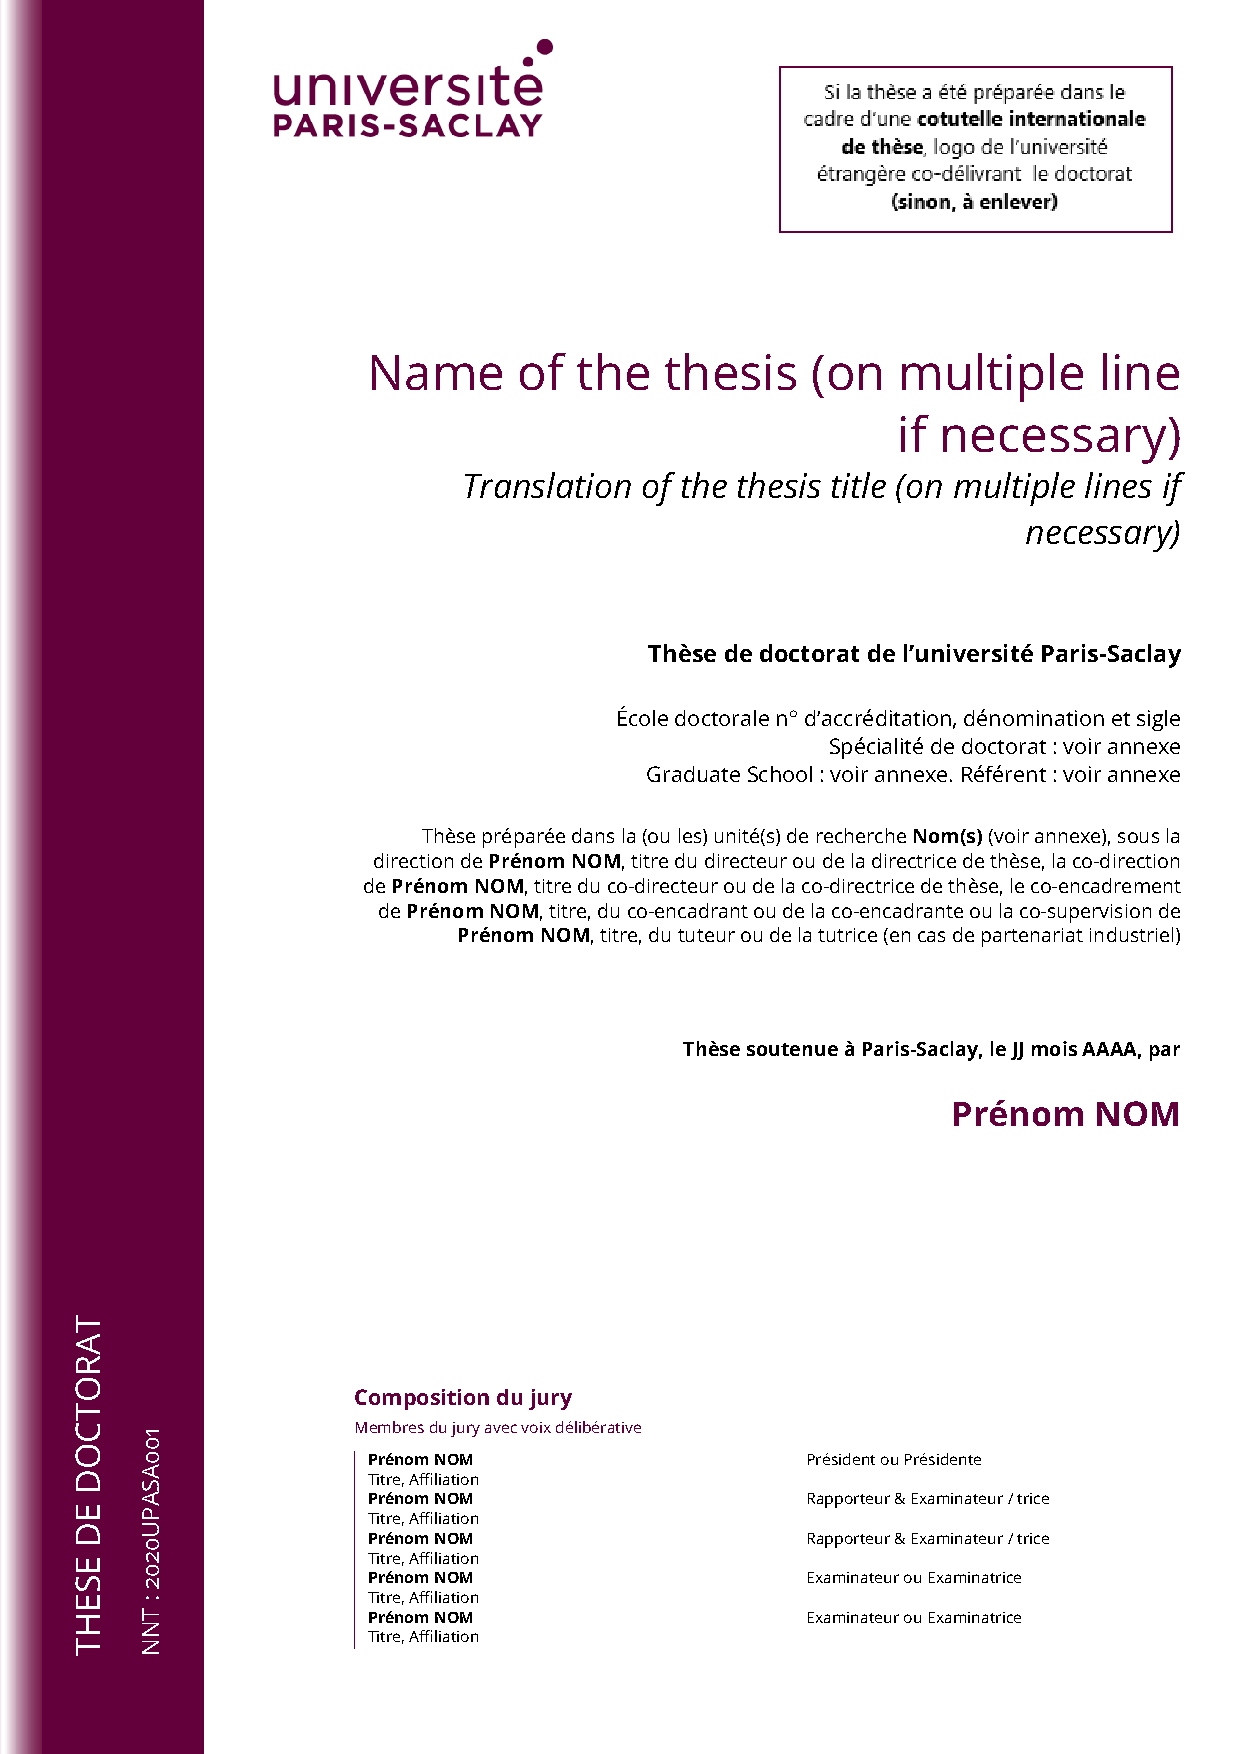
\includepdf[pages=-]{pdfs/titlepage.pdf}    % Include the title page
\setcounter{page}{1}                        % Reset the page counter
% Frontmatter
\addcontentsline{toc}{chapter}{Front Matter}
\mtcaddchapter % Fix enabling minitoc to show correctly

\chapter*{Acknowledgements}
\addcontentsline{toc}{section}{Acknowledgements}

% Table of contents
\cleardoublepage
\phantomsection%
\addcontentsline{toc}{section}{Contents}
\tableofcontents

% List of tables
\cleardoublepage
\phantomsection%
\addcontentsline{toc}{section}{\listtablename}
\listoftables

% List of figures
\cleardoublepage
\phantomsection%
\addcontentsline{toc}{section}{\listfigurename}
\listoffigures

% List of notations
\cleardoublepage
\phantomsection%
\addcontentsline{toc}{section}{List of Symbols}  
\listofnotations

\cleardoublepage


%%% Main matter
\mainmatter

% Introduction
\thesisintroduction{Introduction}

\section{My first section in the introduction}%
\label{sec:my_first_section_in_the_introduction}
\lipsum[1]

\section{My second section in the introduction}%
\label{sec:my_second_section_in_the_introduction}
\lipsum[2-4]

\section{My third section in the introduction}%
\label{sec:my_third_section_in_the_introduction}
\lipsum[2-4]


\clearpage\null

% Part I (can be removed)
\part{My first part title}

\chapter[Short name of chapter]{This is the very long name of the first chapter. It is too long.}

{\color{lmpsblue} \epigraph{La LATIN-PGD c'est génial !}{Alexandre Daby-Seesaram}}

\begin{chapabstract}
    This is the chapter abstract. You can customize its style by modifying the environment \texttt{chapabstract} in the \texttt{lmpsthesis.cls} file.
    \lipsum[1]
\end{chapabstract}

\minitoc

\section{Presentation of the template}%
\label{sec:presentation_of_the_template}

\subsection{An equation}%
\label{sub:an_equation}

This subsection contains the equation of the harmonic decomposition of an elasticity tensor,
\begin{equation}\label{eq:harmonic_decomposition}
    \ela =
        2 \mu \J +
        \kappa \id{2} \otimes \id{2} +
        \frac{1}{2} (\id{2} \otimes \dev{\dil} + \dev{\dil} \otimes \id{2}) +
        \har
\end{equation}
where
    $\mu$ is the shear modulus,
    $\kappa$ is the bulk modulus,
    $\dev{\dil}$ is the deviatoric part of the dilatation tensor, and
    $\har$ is the harmonic part.
Moreover, $\id{2}$ is the second order identity tensor and $\J$ is the deviatoric projector.
You can refer to this equation using the package \texttt{cleveref}\footnote{Guide to \texttt{cleveref}: \url{https://texblog.org/2013/05/06/cleveref-a-clever-way-to-reference-in-latex/}.}.
The \cref{eq:harmonic_decomposition} contains the harmonic decomposition.
\begin{remark}
    The \cref{eq:harmonic_decomposition} uses notations defined in the List of Symbols in the frontmatter.
    Those notations are defined using custom commands in the \texttt{notations.tex} file.
\end{remark}

\subsection{Adding figures}%
\label{sub:adding_figures}

\paragraph{Paragraph with a figure}%
\label{par:paragraph_with_a_figure}
You can insert figures and easily refer to them.
For instance, \cref{fig:c1_cracking_pattern} contains a cracking pattern generated with the \emph{beam-particle} model in the code \texttt{DEAP}.
\begin{figure}
    \centering
    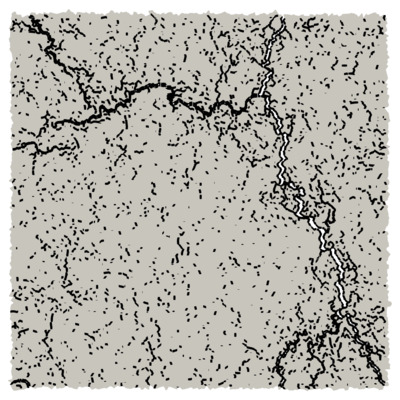
\includegraphics[width=0.3\textwidth]{figures/chapter_1/cracking_pattern_pbc_willam_4.jpg}
    \caption{This is a cracking pattern from DEAP. This file has been compressed to be as small a possible.}
    \label{fig:c1_cracking_pattern}
\end{figure}
We recommend placing images files inside the \texttt{figures} directory.
As you can have a lot of figures, we also recommend making a subdirectory for each chapter.

\paragraph{Paragraph with a tikzpicture}%
\label{par:paragraph_with_a_tikzpicture}
You can also add figures using Tikz.
To use Tikz and PGFPlots in this template, you must activate the option \texttt{tikz} in the definition of the document at the beginning of the file \texttt{PhD\_Thesis.tex}.
\Cref{fig:c1_illustrations_symmetry_classes} contains an illustration of the symmetry classes of elasticity tensors in 2D using Tikz.
\begin{figure}
    \centering
    \tikzsetnextfilename{c1_illustrations_symmetry_classes}
    \begin{tikzpicture}[
        header/.style={align=right, minimum height=1cm, text width=2.5cm},
        cell/.style={align=center, minimum height=2em, minimum width=2cm},
    ]
    % Create a matrix
    \matrix [column sep=0.3cm] {
        % Symmetry classes
        \node[header] {\textbf{Classes}};  &
        &
        \node[cell] (bic) {Biclinic};               &
                                                    &
        \node[cell] (ort) {Orthotropic};            &
                                                    &
        \node[cell] (cub) {Tetragonal};             &
                                                    &
        \node[cell] (iso) {Isotropic};              \\
        % Groups
        \node[header] {\textbf{Groups}};            &
        &
        \node[cell] (zz2) {$\ZZ_2$};                &
        \node {$\subset$};                          &
        \node[cell] (dd2) {$\DD_2$};                &
        \node {$\subset$};                          &
        \node[cell] (dd4) {$\DD_4$};                &
        \node {$\subset$};                          &
        \node[cell] (oo2) {$\OO(2)$};               \\
        % Geometric figures
        \node[header] {\textbf{Illustrations}}; &
        &
        \fill[black] (0,0) circle (0.5pt); \draw (-0.6-0.2,-0.4) -- (-0.6+0.2,0.4) -- (0.6+0.2,0.4) -- (0.6-0.2,-0.4) -- (-0.6-0.2,-0.4);  &
        &
        \fill[black] (0,0) circle (0.5pt); \draw (-0.6,-0.4) -- (-0.6,0.4) -- (0.6,0.4) -- (0.6,-0.4) -- (-0.6,-0.4);  &
        &
        \fill[black] (0,0) circle (0.5pt); \draw (-0.4,-0.4) -- (-0.4,0.4) -- (0.4,0.4) -- (0.4,-0.4) -- (-0.4,-0.4);  &
        &
        \fill[black] (0,0) circle (0.5pt); \draw (0,0) circle (0.4);                                                 \\
    };
    % Add paths
    \draw[->] (bic) -- (ort);
    \draw[->] (ort) -- (cub);
    \draw[->] (cub) -- (iso);
\end{tikzpicture}

    \caption{A tikz illustration of Symmetry classes and their representative group for 2D elasticity tensors. The illustrations are geometric figures in R2 representative of each of the symmetry classes.}
    \label{fig:c1_illustrations_symmetry_classes}
\end{figure}
\begin{remark}
    If you don't want to use Tikz, you should deactivate the option in the document class at the beginning of the main file.
\end{remark}

\begin{remark}
    Note that \texttt{tikzpicture} is automatically externalized.
    To avoid any issues, we recommend you to name the \texttt{tikzpicture} using the command \texttt{\textbackslash textsetnextfilename}.
\end{remark}


\section{Doing some bibliography}%
\label{sec:doing_some_bibliography}

\paragraph{Citing papers}%
\label{par:Citing papers}
Using \texttt{biblatex}, you can cite different works.
Here is an example with different thesis using the early version of this template, such as \textcite{cherriere_elaboration_2023,caruel_caracterisation_2023,ruda_methode_2023,abdel_hafiz_etude_2023}, and more recent version of this template \parencite{daby-seesaram_towards_2023,loiseau_formulation_2023}.
Here, you can also cite some articles.
For instance, you can refer to the works of \textcite{wurtzer_premiere_2022,ribeiro_nogueira_differential_2024}.
You can also cite paper in parentheses \parencite{ruda_first_2022,daby-seesaram_hybrid_2023}.
The list of references appears at the very end of the document.

\section{Another section}%
\label{sec:Another section}

\subsection{With a first subsection}%
\label{sub:with_a_first_subsection}

\lipsum[2-4]

\subsection{And a second subsection}%
\label{sub:and_a_second_subsection}

\lipsum[2-4]

\begin{chaptersummary}
    \lipsum
\end{chaptersummary}

\clearpage\null

% Part II (can be removed)
\part{My second part title}

% Conclusion
\thesisconclusion{Conclusion and perspectives}

\section{My first section in the conclusion}%
\label{sec:my_first_section_in_the_conclusion}
\lipsum[1]

\section{My second section in the conclusion}%
\label{sec:my_second_section_in_the_conclusion}
\lipsum[2-4]

\section{My third section in the conclusion}%
\label{sec:my_third_section_in_the_conclusion}
\lipsum[2-4]


\clearpage\null

% Appendices
\thesisappendix

\chapter{My first appendix}%
\label{cha:my_first_appendix}


\lipsum

\lipsum

\lipsum

\clearpage\null

%%% Backmatter
\backmatter
% Display the bibliography
\printbibliography[heading=bibintoc]

\end{document}

